Das hier aufgelistete Beispiel kann wie in Kapitel \ref{ch:programmeingaben} erklärt, über den Menüeintrag "'Datei"' importiert werden.

\subsection{Format}
Das Format der in den CSV-Dateien gespeicherten Produkte ist zweckmäßig gehalten. Die Werte aller Variablen eines Produkts befinden sich in derselben Zeile. Die Anzahl der Zeilen entspricht somit der Anzahl der zu importierenden Produkte. Die Reihenfolge der Variablenwerte pro Produkt ist folgende:
\begin{compactitem}
	\item Zeilenindex k
	\item Nachfragerate D
	\item Produktionsrate p
	\item Rüstzeit $\tau$
	\item Rüstkostensatz s
	\item Lagerkostensatz h
\end{compactitem}
Die einzelnen Werte werden dabei jeweils durch ein Semikolon voneinander getrennt.

\subsection{Beispiel: Fallstudie Tempelmeier}
Folgende Daten wurden aus \cite{Templ09} entnommen:
\begin{table}[H]
\begin{center}
\begin{tabular}{llllll}
\hline
\multicolumn{1}{|l|}{k} & \multicolumn{1}{l|}{$D_k$} & \multicolumn{1}{l|}{$p_k$} & \multicolumn{1}{l|}{${\tau}_k$} & \multicolumn{1}{l|}{$s_k$} & \multicolumn{1}{l|}{$h_k$} \\ \hline
1                       & 10.4                      & 128.5714                  & 2.0000                          & 190                       & 0.000689                  \\
2                       & 0.8                       & 32.43243                  & 2.0000                          & 210                       & 0.010280                  \\
3                       & 3.6                       & 40.44944                  & 2.0000                          & 140                       & 0.021853                  \\
4                       & 12.22222                  & 51.42857                  & 2.0000                          & 100                       & 0.005105                  \\
5                       & 2.666667                  & 55.38462                  & 2.0000                          & 150                       & 0.005920                  \\
6                       & 4                         & 40.90909                  & 2.0000                          & 110                       & 0.004753                  \\
7                       & 12.44444                  & 45.56962                  & 2.0000                          & 160                       & 0.003530                 
\end{tabular}
\caption[Daten aus \cite{Templ09}]{Daten aus \cite{Templ09}}
\end{center}
\end{table}
Der Inhalt der CSV-Datei hierzu sieht folgendermaßen aus:
\begin{figure}[H]
	\centering
	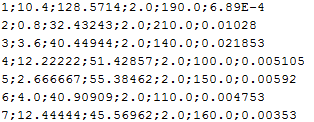
\includegraphics[width=0.5\linewidth]{Bilder/Export.png} 
	\captionof{figure}[Daten aus \cite{Templ09}]{Daten aus \cite{Templ09}}
	\label{fig:export}
\end{figure}
